\question {
    写一个两线程程序,两线程同时向一个数组分别写入$1000$万以内的奇数和偶数,写入过程中两个线
    程共用一个偏移量{ \tt index},代码逻辑如下所示。写完后打印出数组相邻两个数的最大绝对差值。
}
\begin{lstlisting}[language=C]
    int MAX=10000000;
    index = 0
    // thread1
    for (i = 0; i < MAX; i += 2) {
        data[index] = i;     // even(i+1 for thread 2)
        index++;
    }
    // thread2
    for (i = 0; i < MAX; i += 2) {
        data[index] = i + 1; // odd
        index++;
    }
\end{lstlisting}

请分别按下列方法完成一个不会丢失数据的程序:
\begin{enumerate}
    \item 请用{\tt Peterson}算法实现上述功能;
    \item 请学习了解{\tt pthread_mutex_lock/unlock()}函数, 并实现上述功能;
    \item 请学习了解{\tt __atomic_add_fetch}({\tt gcc} $ > 4.7$)或者{\tt C++}中的{\tt std::atomic}类型和{\tt fetch_add()}函数, 并实现上述功能。
\end{enumerate}

提交:
\begin{parts}
    \part 说明你所写程序中的临界区(注意:每次进入临界区之后,执行$200$次操作后离开临界区)
    \part 提供上述三种方法的源代码,运行结果截图(即,数组相邻两个数的最大绝对差值)
    \part 请找一个双核系统测试三种方法中完成数组写入时,各自所需的执行时间,不用提供计算绝对差值的时间
\end{parts}

\begin{solution}
\begin{parts}

% 1
\part
以{\tt Peterson}算法下奇数求和的线程为例,临界区如下所示,已经用注释标注:

\newpage

\begin{lstlisting}[language=C]
#define MAX   10000000
#define TIMES 200
int data[MAX];
int idx = 0;
void* thread2(void* arg) {
    for (int i = 0; i < MAX; i += TIMES * 2) {
        lock_acquire(1);
        /* ========= critical section ============ */
        for (int j = i; j < i + TIMES * 2; j += 2) {
            data[idx] = j + 1;
            idx++;
        }
        /* ========= critical section ============ */
        lock_release(1);
    }
    pthread_exit(NULL);
}
\end{lstlisting}


% 2
\part

{\tt Peterson}算法的源代码如下所示:
\lstinputlisting[language=C]{code/peterson.c}
输出如下:
\begin{figure}[H]
    \centering
    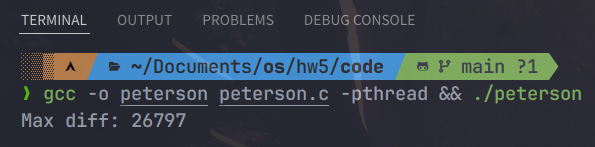
\includegraphics[width=0.6\textwidth]{img/peterson.png}
    \caption{{\tt Peterson}算法输出结果}
\end{figure}

使用{\tt pthread\_mutex\_lock/unlock()}函数的源代码如下所示:
\lstinputlisting[language=C]{code/mutex.c}
输出如下:
\begin{figure}[H]
    \centering
    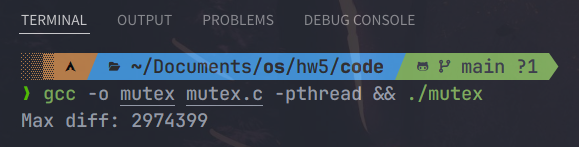
\includegraphics[width=0.6\textwidth]{img/mutex.png}
    \caption{使用{\tt pthread\_mutex\_lock/unlock()}函数输出结果}
\end{figure}

使用{\tt __atomic_add_fetch()}函数的源代码如下所示:
\lstinputlisting[language=C]{code/atomic.c}
输出如下:
\begin{figure}[H]
    \centering
    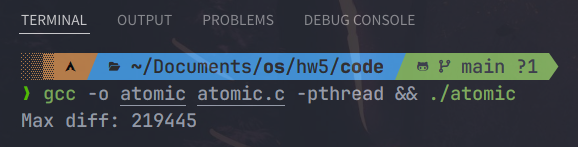
\includegraphics[width=0.6\textwidth]{img/atomic.png}
    \caption{使用{\tt __atomic_add_fetch()}函数输出结果}
\end{figure}


%3
\part
实现双核系统,只需要将两个线程绑定在不同的核上即可,如下所示:

\begin{lstlisting}[language=C]
    void* thread(void* arg) {
        cpu_set_t cpuset;
        CPU_ZERO(&cpuset);
        CPU_SET(0, &cpuset);
        pthread_setaffinity_np(pthread_self(), sizeof(cpu_set_t), &cpuset);
        ...
        pthread_exit(NULL);
    }
\end{lstlisting}

此外再添加记时功能,一共测试$1000$次,取平均值:

\begin{lstlisting}[language=C]
    #define TEST_TIMES 1000
    int main (void) {
        for (int i = 0; i < TEST_TIMES; i++) {
            struct timespec start, end;
            clock_gettime(CLOCK_THREAD_CPUTIME_ID, &start);
            ...
            clock_gettime(CLOCK_THREAD_CPUTIME_ID, &end);
            seperate_time[i] = (end.tv_sec - start.tv_sec) * 1e9 + (end.tv_nsec - start.tv_nsec);
        }
        int total_time = 0;
        int avg_time;
        for (int i = 0; i < TEST_TIMES; i++)
            total_time += seperate_time[i];
        avg_time = total_time / TEST_TIMES;
        printf("Average time: %d ns\n", avg_time);
        return 0;
    }
\end{lstlisting}


最终结果如下:

\begin{figure}[H]
    \centering
    \begin{minipage}{0.6\textwidth}
        \centering
        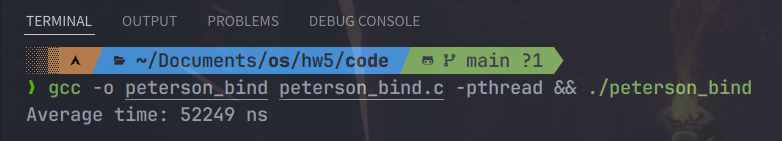
\includegraphics[width=\textwidth]{img/peterson_bind.png}
    \end{minipage}
    \begin{minipage}{0.6\textwidth}
        \centering
        \vspace{1em}
        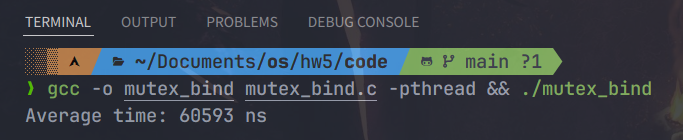
\includegraphics[width=\textwidth]{img/mutex_bind.png}
    \end{minipage}
    \begin{minipage}{0.6\textwidth}
        \centering
        \vspace{1em}
        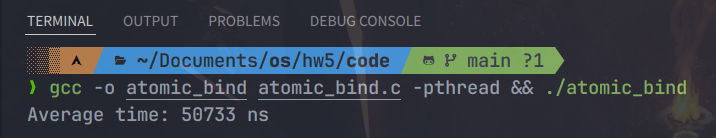
\includegraphics[width=\textwidth]{img/atomic_bind.png}
    \end{minipage}
    \caption{三种方法不同的平均用时}
\end{figure}

可见,{\tt pthread\_mutex\_lock/unlock()}函数的平均用时最长,{\tt Peterson}算法次之, \\
而{\tt \_\_atomic\_add\_fetch()}函数的平均用时最短。

\end{parts}
\end{solution}
